\chapter{Benchmarking QUBO solvers}\label{benchmark}

\section{Related benchmarking work}
One of the first benchmarking works for quantum annealing was conducted by Denchev et al. \yrcite{denchev2016computational}, who measured the performance of D-Wave quantum annealing on the older D-Wave 2X machine using specially crafted problems that have tall and narrow energy barriers separating local minima. Quantum annealing is expected to be $1.8 \times 10^8$ times faster compared to simulated annealing, which tends to fail with problems with such an energy landscape.


\outcite{b34} evaluated the performance of QAOA on the IBMQ backend and the D-Wave quantum annealer using instances of MaxCut and 2-satisfiability problems with up to 18 variables. The performance of the QAOA algorithm is inconsistent and underperforms quantum annealing in their problem set. More recently, \outcite{b35} also compared the performance of QAOA on the IBMQ backend and D-Wave quantum annealing on randomly generated Ising problems with cubic interaction terms and also found that quantum annealing had superior performance over QAOA for all problem sizes. 

\outcite{gomes2019classical} showed that the NNQS solver with an RBM architecture produces good solutions for the max-cut problem with graph sizes of up to 256. \outcite{khandoker2023supplementing} uses recurrent neural networks as the NNQS architecture for the max-cut and traveling salesman problem and found that it outperforms SA. However, there is no direct study that compares performance across QA, QAOA, NNQS, and SA.

\section{Results and Discussion}
Increase to 500 for classic solvers.

\subsection{NAE3SAT}
\begin{figure}[!h]
    \centering
    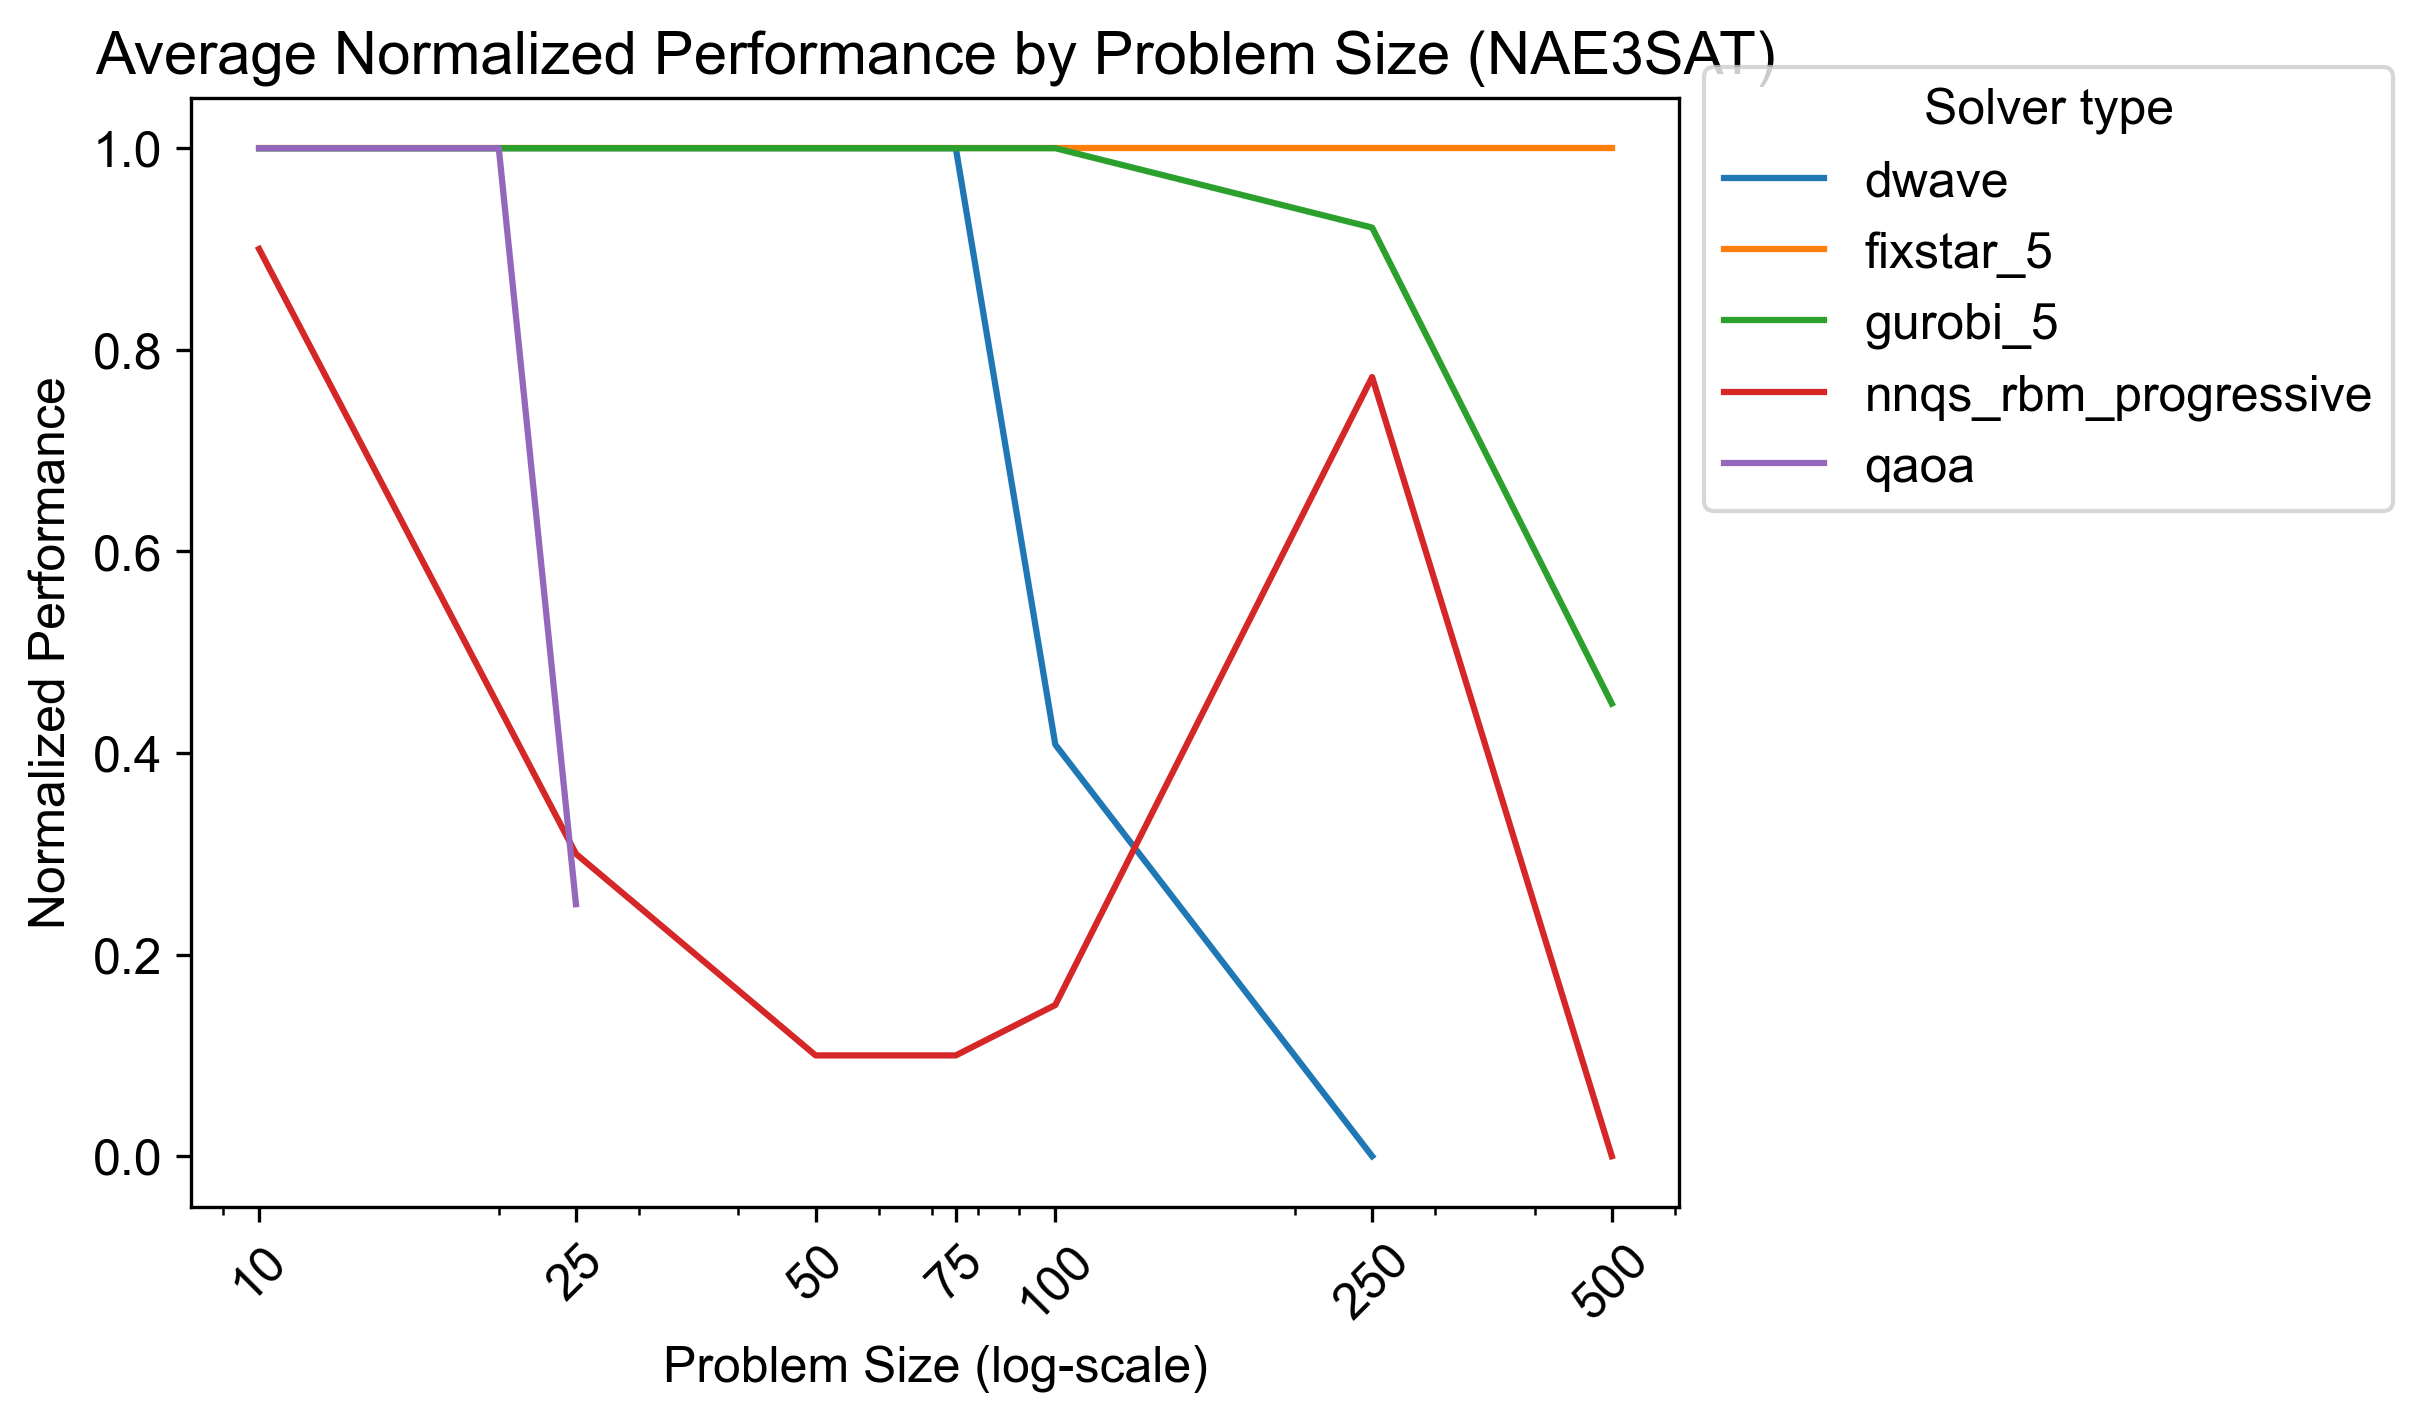
\includegraphics[width=1\linewidth]{images/nae3sat_normalized_performance_all.png}
    \caption{Normalized performance by size on the NAE3SAT dataset}
    \label{all-nae3sat-size}
\end{figure}

\subsection{Max-cut}
\begin{figure}[!h]
    \centering
    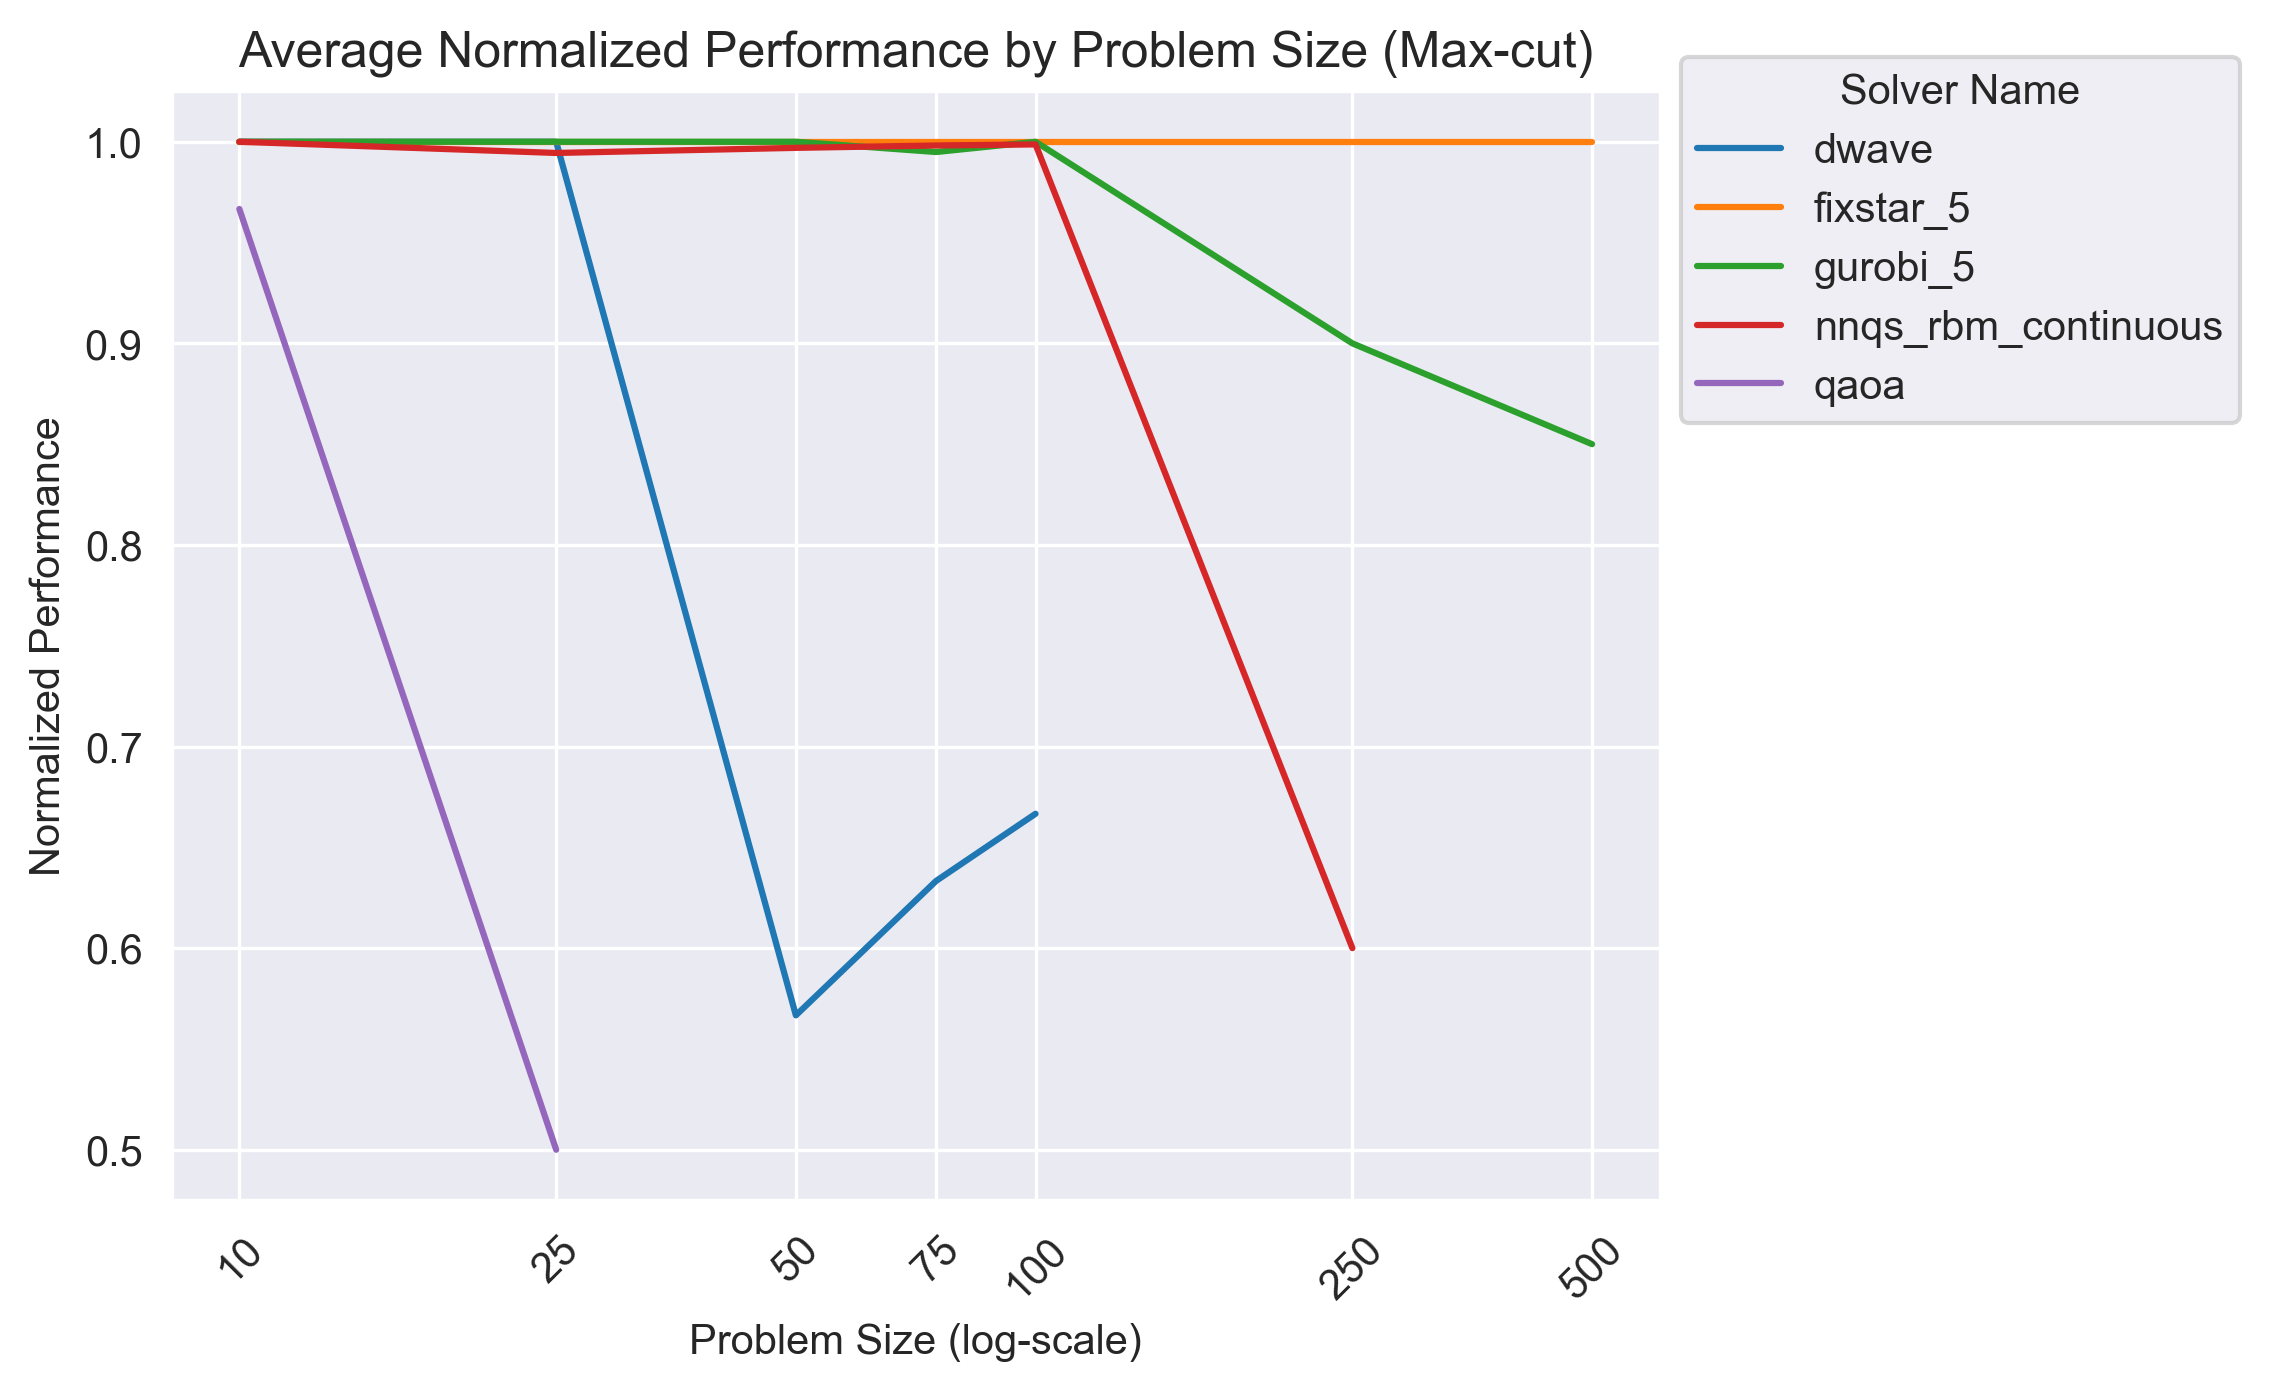
\includegraphics[width=1\linewidth]{images/maxcut_normalized_performance_all.png}
    \caption{Normalized performance by size on the max-cut dataset}
    \label{all-maxcut-size}
\end{figure}

\subsection{SK model}
\begin{figure}[!h]
    \centering
    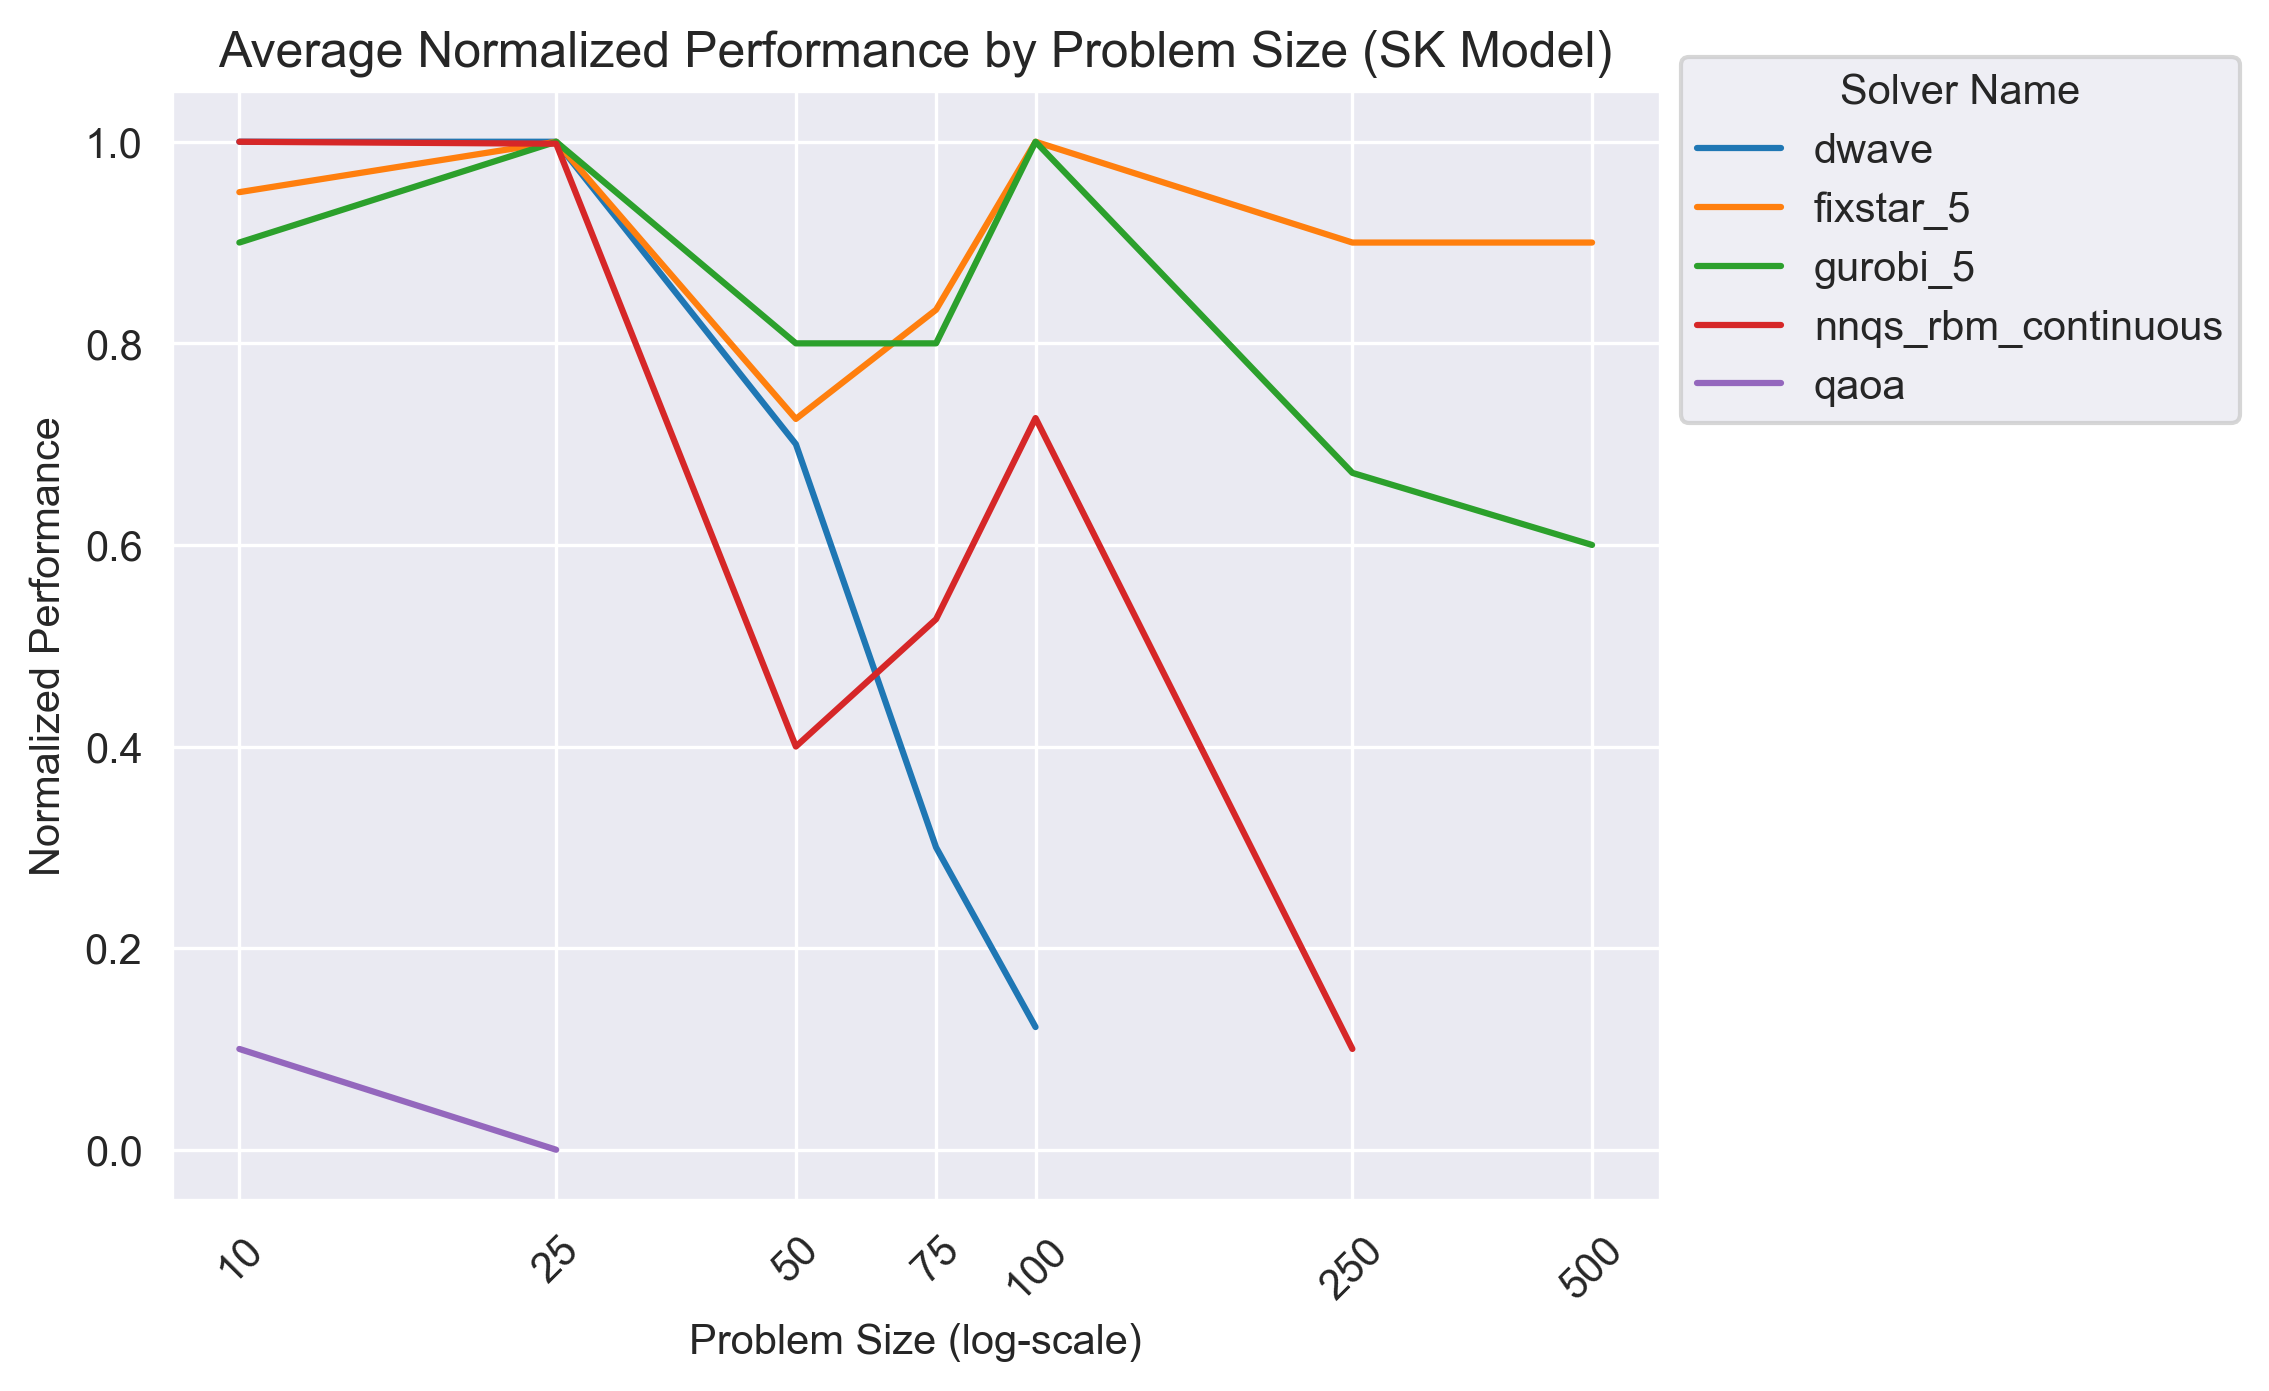
\includegraphics[width=1\linewidth]{images/skmodel_normalized_performance_all.png}
    \caption{Normalized performance by size on the SK model dataset}
    \label{all-skmodel-size}
\end{figure}

\section{Future Work}
Future studies can explore more QUBO problem types and attempt to classify problems that are difficult for annealing-based solvers such as QA and SA but easier for other solvers such as QAOA.